% !TEX options=--shell-escape
%!TEX program = xelatex
\documentclass[11pt,a4paper]{dlove}

\title{\bfseries 基本无害的经济学 \LaTeX{} 技巧}
\author{\href{https://ddswhu.me/}{\bfseries 邓东升} \\  Elegant\LaTeX{} 项目组}
\date{2019 年 11 月 05 日}


\begin{document}


\maketitle

此文档为经济学专业的 \LaTeX{} 技巧总结,包括环境搭建、基础知识、参考文献以及幻灯片制作等内容,仅作为经济学专业的师生作为入门 \LaTeX{} 使用。使用 \mintinline{tex}{dlove} \heart{} 模板和 \hologo{XeLaTeX} 编译完成。

\section{环境搭建}
目前 \LaTeX{} 的主要发行版本如下:
\begin{itemize}
  \item \hologo{MiKTeX}:Windows 上的发行版,国内的 C\TeX{}\footnote{已过时,请尽量不要使用。} 使用的就是 \hologo{MiKTeX};
  \item \TeX{} Live:编辑器 \TeX{}works,跨系统,每年更新一个大版本,最新版为 TeX Live 2019;
  \item Mac\TeX{}:Mac 上的 \TeX{} Live,为了适应 Mac 系统做了一些细微的调整;
\end{itemize} 

推荐使用 \TeX{} Live 2019,可以使用默认的 \TeX{}works 或者配合其他编辑器(比如 Sublime Text、Visual Studio Code)的插件进行编写,后面我们会细说这部分。

\subsection{安装 \TeX{} Live}
首先,我们进入 \TeX{} Live 的\href{https://www.tug.org/texlive/}{官网}地址,点击页面中的 \href{https://www.tug.org/texlive/acquire-netinstall.html}{download},然后可以选择在线安装或者下载安装文件之后离线安装,推荐使用离线安装。
\begin{itemize}
  \item \textbf{在线安装}:点击 \href{http://mirror.ctan.org/systems/texlive/tlnet/install-tl-windows.exe}{install-tl-windows.exe}(Windows) 或者 \href{http://mirror.ctan.org/systems/texlive/tlnet/install-tl-unx.tar.gz}{install-tl-unix.tar.gz}(Linux/Unix),视自己系统选择,然后按照提示进行安装。
  \item \textbf{离线安装}:首先下载镜像文件,点击 \href{https://ctan.org/mirrors}{generic mirror.ctan.org url},这个时候我们会跳转到 \TeX{} Live 的\href{https://ctan.org/mirrors}{镜像站},下拉找到国内的镜像站。在国内的镜像列表中,选择离自己比较近的地区的镜像进行下载\footnote{比如上海的用户可以选择\href{https://mirrors.sjtug.sjtu.edu.cn/ctan/}{上海交大的镜像地址},然后往上拉找到 \TeX{} Live,点击进入上海交大 \TeX{} Live 的\href{https://mirrors.sjtug.sjtu.edu.cn/ctan/systems/texlive/}{下载地址},选择 \href{https://mirrors.sjtug.sjtu.edu.cn/ctan/systems/texlive/Images/}{./images/},然后将 \href{https://mirrors.sjtug.sjtu.edu.cn/ctan/systems/texlive/Images/texlive.iso}{texlive.iso}下载即可。}。下载镜像文件之后,使用资源管理器或者镜像挂载工具\footnote{推荐使用 \href{http://wincdemu.sysprogs.org/}{WinCDEmu} 进行挂载,WinCDEmu 下载后直接安装即可,这里不再赘述。}进行挂载,\textsf{\textcolor{FireBrick}{请不要使用压缩软件对镜像文件解压缩}}。
\end{itemize}

更多的关于 \TeX{} Live 的安装问题,可以参考\href{https://github.com/OsbertWang}{啸行}的\href{https://github.com/OsbertWang/install-latex}{一份简短的关于 \LaTeX{} 安装的介绍}。

\subsection{配置编译环境}
在安装好 \TeX{} Live 之后,我们需要选择一个编辑器,目前主流的编辑器有:
\begin{itemize}
  \item \href{http://www.winedt.com/}{WinEdt},\TeX{} 专用,过去 Windows 上非常流行的编辑器,收费软件,编辑方便,有输入辅助面板,编码支持不好,适合新手,但不推荐;
  \item \href{http://texstudio.sourceforge.net/}{\TeX{}studio},\TeX{} 专用,开源软件,兼顾了易用性以及可定制性,代码提示优秀,有输入辅助面板,适合新手,推荐全阶段使用。
  \item \TeX{}works,\TeX{} 专用,\TeX{} Live 自带的编辑器,界面非常简洁,对于新手不友好,自动补全功能还可以,需要的可以参考我之前的一个总结:\href{https://github.com/EthanDeng/texworks-autocomplete}{\TeX{}works 自动补全功能},推荐不想安装额外软件的用户。
  \item \href{http://www.sublimetext.com/}{Sublime Text},颜值很高、高可定制化的文本编辑器,非 \TeX{} 专用,付费软件,界面非常简洁,自动补全功能完善,代码高亮非常优秀,支持自定义代码片段,插件开发成熟,极度不适合新手,另外插件安装可能受限,极度不适合无法科学上网的用户,只适合高玩以及颜值主义者。
  \item Visual Studio Code, 微软推出的高可定制化文本编辑器,非 \TeX{} 专用,免费软件。可配置快捷编译按钮,自动补全、代码高亮很优秀,插件体验良好,但由于处于不断更新迭代过程,中间可能会有重大改动,需要关注开发者。推荐熟悉 \LaTeX{} 的用户使用。
\end{itemize}

我在我的小圈子里做了一个 \LaTeX{} 编辑器体验调查,表~\ref{tab:editor} 列出了各个编辑器的用户平均评分,此表为主观打分,仅供参考。此表的绘制参考了~\cite{jake2019} 的 \TikZ{} 代码。如果你对这些编辑器有自己的评价,欢迎 \href{https://github.com/EthanDeng/mhlatex4econ/blob/master/archive/LaTeX 编辑器对比评分表.xlsx}{下载评分表},对自己熟悉的编辑器打分,然后发给我 \email{ddswhu@outlook.com},我将加入到这个评分表中。

\begin{table}[htbp]
  \centering
  \caption{\LaTeX{} 编辑器对比}
    \begin{tabular}{cccccc}
    \toprule
             &  WinEdt      &  \TeX{}studio  & \TeX{}works   &  Sublime Text &  VS Code     \\
             \cline{5-6}
    插件依赖  &        &   &  &  \href{https://latextools.readthedocs.io/en/latest/}{\LaTeX{}Tools} &  \href{https://marketplace.visualstudio.com/items?itemName=James-Yu.latex-workshop}{\LaTeX{} Workshop}   \\
    \midrule
    主流系统  &  Win          &  全平台        & Linux/Win     &  全平台        &  全平台       \\
    软件类型  &  商业软件      &  开源软件       & 开源软件       &  商业软件       &  商业软件     \\
    软件价格  &  \href{https://item.taobao.com/item.htm?id=551105790596}{219 元}       &  0             &  0            &  \href{https://www.sublimehq.com/store/text}{80 美元}        &  0           \\
    授权方式  &  终身/教育     &               &               &  终身/个人      &               \\
    % 附加信息  &  教育版本      &               &               &  三年更新       &               \\
    代码高亮  &  \stars{2.7}  &  \stars{3.2}  &  \stars{1.5}  &  \stars{4.3}  &  \stars{4.5}  \\
    颜色主题  &  \stars{2.3}  &  \stars{2.2}  &  \stars{1.0}  &  \stars{4.0}  &  \stars{4.0}  \\
    自动补全  &  \stars{2.7}  &  \stars{3.4}  &  \stars{2.0}  &  \stars{3.5}  &  \stars{4.0}  \\
    代码片段  &  \stars{2.7}  &  \stars{2.4}  &  \stars{0.5}  &  \stars{3.8}  &  \stars{4.0}  \\
    辅助输入  &  \stars{4.0}  &  \stars{3.4}  &  \stars{0.5}  &  \stars{2.3}  &  \stars{3.3}  \\
    开发完成  &  \stars{4.0}  &  \stars{3.8}  &  \stars{4.5}  &  \stars{3.5}  &  \stars{4.0}  \\
    推荐指数  &  \stars{2.7}  &  \stars{4.0}  &  \stars{1.5}  &  \stars{3.0}  &  \stars{4.3}  \\
    \bottomrule
    \end{tabular}%
  \label{tab:editor}%
\end{table}%


\section{基础知识}

\subsection{最简示例}
\begin{code}
\documentclass{article}
% 导言区
\begin{document}
Hello World.
\end{document}
\end{code}
\begin{preview}
Hello World.
\end{preview}

\subsection{中文支持}
目前流行的中文支持有两个方式:
\begin{itemize}
\item \mintinline{tex}{ctex} 宏包,或者与其相适应的 \mintinline{tex}{ctexart} 等文类。
\item \mintinline{tex}{xeCJK} 宏包,需要使用 \hologo{XeLaTeX} 编译。
\end{itemize}

\subsection{数学字母}
常用的一些希腊字母见表~\ref{tab:greek_letters},需要注意的是这些希腊字母需要在数学模式(比如 \mintinline{tex}{$\alpha$})或者数学环境中使用。
\begin{table}[htbp]
  \centering
  \small
  \caption{希腊字母表}
    \begin{tabular}{llllll}
    \toprule
    \textsf{符号} & \textsf{命令} & \textsf{符号} & \textsf{命令} & \textsf{符号} & \textsf{命令} \\
    \midrule
    $\alpha$ & \mintinline{tex}{\alpha} & $\iota$ & \mintinline{tex}{\iota} & $\sigma$\; $\Sigma$ & \mintinline{tex}{\sigma \Sigma} \\
    $\beta$ & \mintinline{tex}{\beta} & $\kappa$ & \mintinline{tex}{\kappa} & $\tau$ & \mintinline{tex}{\tau} \\
    $\gamma$\; $\Gamma$ & \mintinline{tex}{\gamma \Gamma} & $\lambda$ \; $\Lambda$ & \mintinline{tex}{\lambda \Lambda} & $\upsilon$\; $\Upsilon$ & \mintinline{tex}{\upsilon \Upsilon} \\
    $\delta$ \; $\Delta$ & \mintinline{tex}{\delta \Delta} & $\mu$ & \mintinline{tex}{\mu} & $\phi$\; $\Phi$ & \mintinline{tex}{\phi \Phi} \\
    $\epsilon$ & \mintinline{tex}{\epsilon} & $\nu$ & \mintinline{tex}{\nu} & $\chi$ & \mintinline{tex}{\chi} \\
    $\zeta$ & \mintinline{tex}{\zeta} &  $\pi$ \; $\Pi$& \mintinline{tex}{\pi \Pi} & $\psi$\; $\Psi$ & \mintinline{tex}{\psi \Psi} \\
    $\eta$ & \mintinline{tex}{\eta} & $\rho$ & \mintinline{tex}{\rho}  & $\omega$\; $\Omega$ & \mintinline{tex}{\omega \Omega} \\
    $\theta$ & \mintinline{tex}{\theta} & $\varepsilon$ &  \mintinline{tex}{\varepsilon} &       &  \\
    \bottomrule
    \end{tabular}%
  \label{tab:greek_letters}%
\end{table}%

\subsection{文本模式与数学模式}
在 \LaTeX{} 中,文本和数学是作为两个独立的不同模式存在的,如果需要在文本模式中输入数学式,需要使用英文状态下的美元符号 \mintinline{tex}{$} 将数学命令包围,比如 \mintinline{tex}{$\alpha$} 输出为 $\alpha$。

\begin{code}
假设 $y_{i}$ 是被解释变量的第 $i$ 次观测,$x_{i}$ 是解释变量的第 $i$ 次观测,设定回归方程为 $y_{i} = \alpha + \beta x_{i} + \varepsilon_{i}$。
\end{code}
\begin{preview}
假设 $y_{i}$ 是被解释变量的第 $i$ 次观测,$x_{i}$ 是解释变量的第 $i$ 次观测,设定回归方程为 $y_{i} = \alpha + \beta x_{i} + \varepsilon_{i}$。
\end{preview}

\subsection{数学环境}
数学环境中,最简单的就是 \mintinline{tex}{equation} 环境,这个环境会对数学公式进行自动编号,如果不需要编号,可以使用 \mintinline{tex}{equation*} 环境。\par

\begin{code}
\begin{equation}
y_{i} = \alpha + \beta x_{i} + \varepsilon_{i}
\end{equation}
\end{code}
\begin{preview}
\begin{equation}
y_{i} = \alpha + \beta x_{i} + \varepsilon_{i}
\end{equation}
\end{preview}

\section{表格输入}
\LaTeX{} 中表格的输入并不太方便,最简单的一个表格示例如下:

\begin{code}
\begin{tabular}{ccc}
  English &  Context &   996   \\ 
  Right   &   Here   &  1024   \\ 
  Chinese & $\alpha$ & $\beta$ \\   
\end{tabular}
\end{code}
\begin{preview}
\begin{center}
\begin{tabular}{ccc}
  English &  Context &   996   \\ 
   Right  &   Here   &  1024   \\ 
  Chinese & $\alpha$ & $\beta$ \\   
\end{tabular}
\end{center}
\end{preview}

在上述命令中,创建表格的环境名为 \mintinline{tex}{tabular},而 \mintinline{tex}{tabular} 后的选项为列的对齐方式,分别有居中对齐(c),左对齐(l),右对齐(r),而同一行的不同列之间用 \& 隔开,而换行使用 \mintinline{tex}{\\}。很显然,这种表格并不是我们想要的,我们需要加入一些表格框线:

\begin{code}
\begin{tabular}{|l|c|r|} 
  \hline
  English &  Context &     996 \\ 
  Right   &   Here   &    1024 \\ 
  Chinese & $\alpha$ & $\beta$ \\ 
  \hline
\end{tabular}
\end{code}
\begin{preview}
\begin{center}
\begin{tabular}{|l|c|r|} 
  \hline
  English &  Context &     996 \\ 
  Right   &   Here   &    1024 \\ 
  Chinese & $\alpha$ & $\beta$ \\ 
  \hline
\end{tabular}
\end{center}
\end{preview}

可以发现,\mintinline{tex}{|} 为表格的列添加竖线,而 \mintinline{tex}{\hline} 为表格的行添加了横线。

\subsection{三线表}

在实际写作中,我非常推荐大家使用三线表,而不要添加过多的横线或者竖线,利用 \mintinline{tex}{booktabs} 宏包中的 \mintinline{tex}{\toprule}、\mintinline{tex}{\midrule} 以及 \mintinline{tex}{\bottomrule} 能够非常方便的制作出三线表。示例如下:

\begin{code}
\begin{tabular}{lcr}
  \toprule
  Language &   Infor  &  Number \\
  \midrule
  English  &  Context &     996 \\ 
  Right    &   Here   &    1024 \\ 
  Chinese  & $\alpha$ & $\beta$ \\ 
  \bottomrule
\end{tabular}
\end{code}
\begin{preview}
\begin{center}
\begin{tabular}{lcr}
  \toprule
  Language &   Infor  &  Number \\
  \midrule
  English  &  Context &     996 \\ 
  Right    &   Here   &    1024 \\ 
  Chinese  & $\alpha$ & $\beta$ \\ 
  \bottomrule
\end{tabular}
\end{center}
\end{preview}

\subsection{长表格}
如果表格非常长,可以使用 \mintinline{tex}{longtable} 代替 \mintinline{tex}{table}。

\begin{code}
\begin{table}
  \begin{tabular}
    % 表格内容
  \end{tabular}
\end{table}
\end{code}
\hspace{0.02\textwidth}
\textcolor{gray}{\vrule}
\hspace{0.02\textwidth}
\begin{code}
\begin{longtable}
  \begin{tabular}
    % 表格内容
  \end{tabular}
\end{longtable}
\end{code}

\subsection{辅助工具}
手动输入表格是一个非常枯燥的过程,而且容易出错,因此我们推荐借助其他工具辅助制作表格,其中个人体验最好的一个工具是 \href{https://ctan.org/pkg/excel2latex}{Excel2\LaTeX{}}。你可以通过 CTAN 的\href{http://mirrors.ctan.org/support/excel2latex.zip}{下载地址}或者\href{https://github.com/EthanDeng/mhlatex4econ/blob/master/archive/excel2latex.zip}{此处}下载此插件,将插件下载解压缩之后,双击打开即可使用,不过建议把 \mintinline{tex}{Excel2LaTeX.xla} 置于 Excel 的启动文件夹内,这样以后就不用每次查找这个 Excel 宏才能使用。我本人的 Office 是 2019,对应的 Excel 的启动目录为 \mintinline[breaklines]{python}{C:\Program Files\Microsoft Office\root\Office16\XLSTART},如此,在你的 Excel 上方会出现一个插件选项卡,有两个表格转换的选项,见图~\ref{fig:excel2latex}。选中所需要转换的表格,然后选择 \mintinline{shell}{Convert Table to LaTeX} 即可。

\begin{figure}
\centering
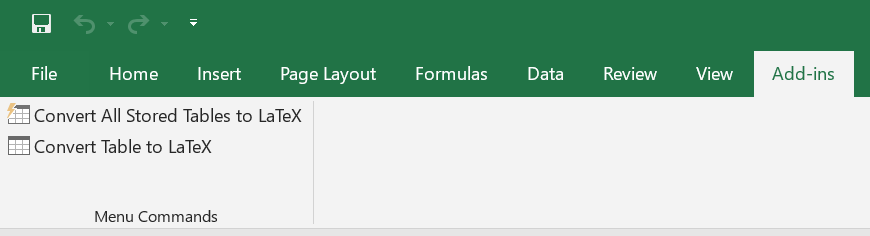
\includegraphics[width=0.6\textwidth]{excel2latex.png}
\caption{Excel2\LaTeX{} 插件\label{fig:excel2latex}}
\end{figure}


另外在线转换的工具 \href{https://tableconvert.com/?output=latex}{Table Convert} 也可以尝试一下。


\subsection{回归表格}

outreg2 

R

Python

\section{颜色}

在 \LaTeX{} 中,有 7 种内置的颜色,分别是 white, black, red, green, blue, cyan, magenta, yellow。

\subsection{定义颜色}

\subsection{使用颜色}

\section{文献}

\subsection{thebibliography 环境}

\subsection{\hologo{BibTeX} 的使用}

\subsection{natbib 包}

\section{幻灯片}
Beamer 是 \LaTeX{} 用于制作幻灯片的一个文类,由于它的格式简洁、易于使用、方便展示数学公式和逻辑演绎,在学术界特别是国外非常受欢迎。下面分别是是英文 Beamer 和中文 Beamer 的一个简单示例:

\begin{code}
\documentclass{beamer}

% title information
\title{An Example of Beamer Class}
\author{Dongsheng DENG}
\institute{Fudan University}
\date{\today}

\begin{document}
\maketitle

\begin{frame}{frame title}
Be honest rather clever.
\end{frame}

\end{document}
\end{code}
\begin{code}
\documentclass{beamer}
\usepackage[UTF8,scheme=plain]{ctex}
% 标题信息
\title{Beamer 文类示例}
\author{邓东升}
\institute{复旦大学}
\date{2019 年 10 月 23 日}

\begin{document}
\maketitle

\begin{frame}{帧标题}
有志者事竟成,百二秦关终属楚。
\end{frame}

\end{document}
\end{code}

\section{文档说明}

本文档使用了 \mintinline{tex}{fontspec} 和  \mintinline{tex}{xeCJK} 设置英文字体和中文字体,用户需要的字体列表如下:
\begin{table}[htbp]
  \centering
  \caption{本文档字体设置}
    \begin{tabular}{lccc}
    \toprule
          & \textbf{衬线字体}  & \textbf{非衬线字体} & \textbf{等宽字体}   \\
    \midrule
    英文/\mintinline{tex}{fontspec}    & Amiri & \textsf{Roboto} & \texttt{Ubuntu Mono} \\
    中文/\mintinline{tex}{xeCJK}   & 方正书宋简体 & \textsf{方正楷体简体} & \texttt{方正仿宋简体}  \\
    \bottomrule
    \end{tabular}%
  \label{tab:fontset}%
\end{table}%

需要注意的是,在 Win 10 中,安装字体时需要\textsf{\textcolor{FireBrick}{为所有用户安装}},否则即便安装了字体,\LaTeX{} 也无法找到。

另外,本文高亮使用了 \mintinline{tex}{minted} 宏包,所以,需要调用 \mintinline{shell}{-shell-escape} 选项并用 \hologo{XeLaTeX} 进行编译,如果使用命令行编译,命令如下:
\begin{minted}{shell}
xelatex --shell-escape main.tex
\end{minted}

\bibliographystyle{plainnat}
\nocite{overleaftables,overleafbibtex}
\bibliography{reference}

\end{document}